\documentclass[11pt,a4paper,notitlepage]{article}
\usepackage[margin = 1.5cm]{geometry}
\usepackage[utf8]{inputenc}
\usepackage{lmodern}
\usepackage[T1]{fontenc} 
\usepackage{microtype}
\usepackage{inconsolata}
\usepackage[icelandic,english]{babel}
\selectlanguage{english}
\usepackage{amsmath}
\usepackage{amsfonts}
\usepackage{amssymb}
\usepackage{amsthm}
\usepackage{enumerate}
\usepackage{multicol}
\usepackage{tasks}
\usepackage{xcolor}
\usepackage{siunitx}
\usepackage{caption}
\usepackage{subcaption}
\usepackage{etoolbox}
\usepackage{graphicx}
\usepackage{float}
\usepackage{booktabs}
\usepackage{tikz}
\usepackage{hyperref}
\hypersetup
{
    colorlinks=true,
    linkcolor=blue,
    citecolor=blue,
    filecolor=blue, 
  	urlcolor=blue,
}
\usepackage[all]{hypcap}
\usepackage{verbatim}
\usepackage{listings}
\lstdefinestyle{java-dark}
{	
    backgroundcolor=\color{black},
    commentstyle=\color{gray},
    keywordstyle=\color{red},
    numberstyle=\tiny\color{black},
    stringstyle=\color{green},
    identifierstyle=\color{orange},
	basicstyle=\scriptsize\ttfamily\color{white},
    breakatwhitespace=false,
    breaklines=true,
    captionpos=b,
    keepspaces=true,
    numbers=left,
    numbersep=5pt,
    showspaces=false,
    showstringspaces=false,
    showtabs=false,
    tabsize=2,
}
\lstdefinelanguage{Sage}[]{Python}
{morekeywords={False,sage,True},sensitive=true}

\newcommand{\B}{\mathbb{B}} % binary set
\newcommand{\N}{\mathbb{N}} % set of natural numbers
\newcommand{\Z}{\mathbb{Z}} % set of integers 
\newcommand{\Q}{\mathbb{Q}} % set of rationals
\newcommand{\R}{\mathbb{R}} % set of reals
\newcommand{\C}{\mathbb{C}} % set of complex
\newcommand{\map}[3]{#1: #2 \to #3} % 1 : 2 -> 3
\newcommand{\der}[1]{\frac{d}{d#1}} % derivative
\newcommand{\set}[1]{\left\{#1\right\}} % set, general
\newcommand{\nset}[1]{\set{1,2,\ldots,#1}} % {1,2,...,n}
\newcommand{\cata}[1]{\frac{1}{#1+1}\binom{2#1}{#1}} % catalan numbers
\renewcommand{\vector}[1]{(x_1,x_2,\ldots,x_{#1})} % x-vector, len n
\newcommand{\avector}[2]{(#1_1,#1_2,\ldots,#1_{#2})} % ?-vector, len n
\newcommand{\vvec}[1]{\begin{pmatrix}#1\end{pmatrix}}
\newcommand{\mc}[1]{\mathcal{#1}}
\newcommand{\ttt}[1]{\texttt{#1}}
\newcommand{\ilim}[1]{\lim_{#1\to\infty}}
\newcommand{\bpar}[1]{\left(#1\right)}
\newcommand{\floor}[1]{\left\lfloor #1 \right\rfloor}
\newcommand{\lerp}[1]{\text{lerp}\left(#1\right)}

\newcommand{\setOutput}
{
\lstset{
  frame=single,
  showtabs=False,
  showspaces=False,
  tabsize=2,
  showstringspaces=False,
  language={},
  basicstyle={\fontsize{10pt}{10pt}\ttfamily},
  numbers=none,
  captionpos=b,
  aboveskip=0.3em,
  belowskip=0.1em
}
}

\newcommand{\maketitlepage}
{
  \begin{titlepage}
    \begin{center}
      \ \\[2.5cm]
      
\includegraphics[width=0.65\textwidth]{rulogo.png}\\[2.5cm]
      \textsc{\Huge Artificial Intelligence}\\[.5cm]
      \textsc{\LARGE Breakthrough - Adversarial Search}\\[1.2cm]
      \textsc{\Large \today}\\[4cm]
      \textsc{\huge Jón Steinn Elíasson}\\[.3cm]      
      \text{jonse07@ru.is}
    \end{center}
    \vfill
  \end{titlepage}
}

\newcommand{\maketocpage}
{
  \tableofcontents
  \listoftables
  \listoffigures
  \lstlistoflistings
  \vfill
  \clearpage
}

\begin{document}
\maketitlepage{}
\maketocpage{}

\section{Introduction}
This project is about implementing an agent to play a variation of Breakthrough. This version only allows diagonal kills which introduces the notion of draws. The board size is also not fixed.\\

A game state is represented by a set of positions for each color. Some other ways of representing the states such as bitboards were explored but seeing as our table size varies, the more simplistic approach of sets was used. A move is represented by a source and destination position, both a two element integer tuple. The agent searches, within the given time limit, until all leaves are terminal leaves.\\

A Negamax variant of alpha beta pruning was used, where ($\alpha$, $\beta$) are passed down as $(-\beta,-\alpha)$ such that each player is always the maximizer when evaluating. He tries to maximize the value which negation is passed to the other player above in the tree.

\section{Board evaluation}
	\subsection{Terminal evaluation}
    	Since white can't move into a black winning state and vice versa, there is no need to check if the current player has won. We only need to check if he has lost or if he has any moves.\\
        
        For the white player we do so by iterating over the set of black positions and check if any has reached a goal position, if so a \texttt{LOST} value is returned. If not, we check if white has any possible movements and if so, return a \texttt{NON\_TERMINAL} value. Otherwise a \texttt{DRAW} variable is returned. Evaluating terminal state for black works similarly. In any expansion, we check for these values to see if we should continue.
        
    \subsection{Player evaluation}\label{ss:pe}
    	Evaluating the board for each player depends on several variables.
        \begin{enumerate}[i.]
        	\item \textbf{Pawn count}. The pawns of each player are counted and multiplied with a count value. In figure \ref{fig:evalCnt}, the white player would get a score of \texttt{3 * count\_value}, while the black would get \texttt{2 * count\_value}. 
\begin{figure}[H]
	\begin{center}
		\begin{tikzpicture}[thick,scale=0.5, every node/.style={scale=0.5}]
			\draw (0,0) grid (6,6);
			\fill (4.5,1.5) circle (0.25);
			\fill (3.5,1.5) circle (0.25);
			\draw (1.5,1.5) circle (0.25);
			\draw (2.5,2.5) circle (0.25);
			\draw (0.5,3.5) circle (0.25);
		\end{tikzpicture}
	\end{center}
	\caption{Count value evaluation}
	\label{fig:evalCnt}
\end{figure}
		\item \textbf{Furthest pawn}. The furthest pawn is multiplied with a furthest value. In figure \ref{fig:evalFar}, the white player has a score of \texttt{4 * furthest\_value} while the black has a value of \texttt{5 * furthest\_value}. The value of black is calculated by subtracting its minimum $y$ position from the table's height plus one while the value for white is his maximum $y$ position.
\begin{figure}[H]
	\begin{center}
		\begin{tikzpicture}[thick,scale=0.5, every node/.style={scale=0.5}]
			\draw (0,0) grid (6,6);
			\fill (4.5,1.5) circle (0.25);
			\draw (3.5,3.5) circle (0.25);
			\draw (3.5,1.5) circle (0.25);
		\end{tikzpicture}
	\end{center}
	\caption{Furthest value evaluation}
	\label{fig:evalFar}
\end{figure}
		\item \textbf{Movable pawns}. For each player, we count the number of pawns he can move and multiply it by a can move value. In figure \ref{fig:evalCnMv}, black can only move the upper left pawn while the white player can move 2, so there evaluation are \texttt{1 * can\_move\_value} and \texttt{2 * can\_move\_value} respectively.
\begin{figure}[H]
	\begin{center}
		\begin{tikzpicture}[thick,scale=0.5, every node/.style={scale=0.5}]
			\draw (0,0) grid (6,6);
			\fill (3.5,4.5) circle (0.25);
			\fill (0.5,5.5) circle (0.25);
			\draw (3.5,3.5) circle (0.25);
			\draw (2.5,2.5) circle (0.25);
			\draw (1.5,4.5) circle (0.25);
		\end{tikzpicture}
	\end{center}
	\caption{Can move value evaluation}
	\label{fig:evalCnMv}
\end{figure}
		\item \textbf{Unhindered pawns}. Here we check whether a pawn has a clear path to the other end. This factor is multiplied with how far it is so the closer to goal the better. It checks each pawn current column (not those behind it) as well as both the columns to the left and right. In figure \ref{fig:evalUnH} we have 2 black pawns and 3 white. The black pawn at $(1,5)$ does not have a clear path because of the white pawn at $(2,1)$ and vice versa. The black pawn at $(4,3)$ does have a clear path to the goal and he is on the forth row counting from his start so we would add $4$ to a variable that is ultimately multiplied with the \texttt{unhindered\_value}. The white pawns at $(4,4)$ and $(6,1)$ have a clear path so we would add 4 and 1 to this variable for white. In the end, this would evaluate to \texttt{4 * unhindered\_value} and \texttt{(4+1) * unhindered\_value} for the black and white players respectively.
\begin{figure}[H]
	\begin{center}
		\begin{tikzpicture}[thick,scale=0.5, every node/.style={scale=0.5}]
			\draw (0,0) grid (6,6);
			\fill (0.5,4.5) circle (0.25);
			\fill (3.5,2.5) circle (0.25);
			\draw (3.5,3.5) circle (0.25);
			\draw (5.5,0.5) circle (0.25);
			\draw (1.5,0.5) circle (0.25);
		\end{tikzpicture}
	\end{center}
	\caption{Unhindered value evaluation}
	\label{fig:evalUnH}
\end{figure}
        \item \textbf{Lane control}. Here we check how many of the columns are occupied by our pawns. In figure \ref{fig:evalLaCtrl} the black has pawns on 5 columns while white only at 4. This would evaluate to \texttt{5 * lane\_control\_value} and \texttt{4 * lane\_control\_value} for black and white respectively.
\begin{figure}[H]
	\begin{center}
		\begin{tikzpicture}[thick,scale=0.5, every node/.style={scale=0.5}]
			\draw (0,0) grid (6,6);
			\fill (2.5,2.5) circle (0.25);
			\fill (1.5,2.5) circle (0.25);
			\fill (0.5,2.5) circle (0.25);
			\fill (1.5,4.5) circle (0.25);
			\fill (5.5,1.5) circle (0.25);
			\fill (4.5,2.5) circle (0.25);
			\draw (1.5,1.5) circle (0.25);
			\draw (4.5,4.5) circle (0.25);
			\draw (0.5,4.5) circle (0.25);
			\draw (3.5,1.5) circle (0.25);
			\draw (4.5,2.5) circle (0.25);
			\draw (3.5,2.5) circle (0.25);
		\end{tikzpicture}
	\end{center}
	\caption{Lane control value evaluation}
	\label{fig:evalLaCtrl}
\end{figure}
	\item \textbf{Win next}. Here we check if the players can win next turn. The value of this attribute is always greater then the maximum gained from the others combined but still less than a negative loss value (and $-\infty$). This takes into account who's turn it is so that the player who's turn it is dominates the other in case both players win next. The value is doubled for the player who's turn it is (in both cases this would dominate all other attributes so this is just for this single scenario). We also take into account that if a player who's turn it is not, has only a single move to a winning position and that being an attack move. If so, we do not look at it as a win next scenario since we assume the other person would kill his piece. If however two such scenario were to arise on the table, the other player could only eliminate one. We must however check, in this case, if we only have two pawns attacking the same piece.\\
    
    The special case is shown for black in figure \ref{fig:winNxtSpec}. If we would not check for this scenario, our evaluation of the state would be that black wins next but in fact this is a winning position for white, starting by moving pawn $(3,1)$ to $(3,2)$ and then just advancing the right most pawn.
\begin{figure}[H]
	\begin{center}
		\begin{tikzpicture}[thick,scale=0.5, every node/.style={scale=0.5}]
			\draw (0,0) grid (6,6);
			\fill (1.5,1.5) circle (0.25);
			\fill (0.5,5.5) circle (0.25);
			\fill (3.5,1.5) circle (0.25);
			\draw (3.5,0.5) circle (0.25);
			\draw (5.5,3.5) circle (0.25);
			\draw (2.5,0.5) circle (0.25);
			\draw (1.5,0.5) circle (0.25);
		\end{tikzpicture}
	\end{center}
	\caption{Win next special case}
	\label{fig:winNxtSpec}
\end{figure}

In the state shown in figure \ref{fig:winNxt}, both players are in a 'win next' position. If it would be white to play, we would evaluate his score as \texttt{2 * win\_next\_value} while only \texttt{1 * win\_next\_value} for the black.
\begin{figure}[H]
	\begin{center}
		\begin{tikzpicture}[thick,scale=0.5, every node/.style={scale=0.5}]
			\draw (0,0) grid (6,6);
			\fill (2.5,5.5) circle (0.25);
			\fill (0.5,5.5) circle (0.25);
			\fill (3.5,1.5) circle (0.25);
			\draw (3.5,4.5) circle (0.25);
			\draw (1.5,4.5) circle (0.25);
		\end{tikzpicture}
	\end{center}
	\caption{Win next for both players}
	\label{fig:winNxt}
\end{figure}
        \end{enumerate}
    \subsection{Heuristic}
    	To evaluate a state for white, we subtract the board evaluation for black if it's not his turn from the evaluation for white if it's his turn. For black, it would be the evaluation for white if not to play subtracted from the evaluation for black if it's his turn.\\
        
        The values assigned to each part of the valuation was done by making two agent compete against each other and the one who lost changed one of his values. All values were kept in $\left[1,500\right]$. More details about that can be found in subsection \ref{ss:h2h}.
    	
    	
\section{Experiments}
\subsection{Head to head}\label{ss:h2h}
A static variable is used to store an instance of values for our heuristic and this variables is used by the agent. Initially all values were set to 1, then two agent would play against each other, one using the stored values and the other choosing one of it's values and increasing it by one. This should be repeated until increasing any value results in a loss.\\

A $8 \times 8$ board was used to play on and the time limit set to 1 second so that the agents would need to relay on their estimate. To make the experiment more reliable, a best out of three system was used as well as choosing color at random. These experiment took very long since the agents do not favor early terminals and in total, several hours went into this (although other work was done while they played out). At the time of the hand in, a search for such a set of values was still ongoing. The method for this experiment (\texttt{testSingleEstimate()}) can be found in the test class \href{https://github.com/JonSteinn/Breakthrough/blob/master/test/agents/MyAgentTest.java}{MyAgentTest}. The resulting values the experiment yielded (so far) can be seen in table \ref{table:valestimp}.

\begin{table}[H]
\begin{center}
\begin{tabular}{c|ccccc}
Variable & count & furthest & movable & unhindered & laneControl \\
\hline
Value & 5 & 8 & 4 & 10 & 2
\end{tabular}
\end{center}
\caption{Improved values for estimates}
\label{table:valestimp}
\end{table}

After finding values for our heuristic, another experiment was conducted where the agent played against another with random values. This was done on a $5 \times 5$ board with 1 second time limit and again, using random colors and a best out of three system. An output example can be seen in listing \ref{lst:ranLose}, appendix \ref{app:h2ho}. The output for the first experiment was identical (but a single entry). The latter experiment method (\texttt{testEstimates()}) can be found in the same class.

\subsection{Expansions}
The alpha beta search was run with no order, simple ordering (priority queue with most advanced pieces first), sorted by heuristic and than using a transposition table and heuristic ordering. All tests were done on a $8 \times 8$ board with a time limit of 10 seconds.
\subsubsection{No ordering}
\begin{table}[H]
	\begin{center}
		\begin{tabular}{c|c|c|c}
			Iteration & Expansions & Depth & Time \\
			\hline
			1 & 9 & 1 & 0 \\
			2 & 24 & 2 & 0 \\
			3 & 103 & 3 & 16 \\
			4 & 246 & 4 & 16 \\
			5 & 1210 & 5 & 31 \\
			6 & 4598 & 6 & 122 \\
			7 & 24368 & 7 & 288 \\
			8 & 90737 & 8 & 842 \\
			9 & 540912 & 9 & 2499 \\
		\end{tabular}
	\end{center}
	\caption{No ordering}
	\label{table:noOrd}
\end{table}
\subsubsection{Order of column position}
\begin{table}[H]
	\begin{center}
		\begin{tabular}{c|c|c|c}
			Iteration & Expansions & Depth & Time \\
			\hline
			1 & 9 & 1 & 88 \\
			2 & 24 & 2 & 15 \\
			3 & 110 & 3 & 12 \\
			4 & 379 & 4 & 18 \\
			5 & 2031 & 5 & 47 \\
			6 & 7148 & 6 & 104 \\
			7 & 37232 & 7 & 461 \\
			8 & 135318 & 8 & 2121 \\
			9 & 748961 & 9 & 3104 \\
		\end{tabular}
	\end{center}
	\caption{Simple ordering (advanced first)}
	\label{table:pqAdv}
\end{table}

\subsubsection{Order by heuristic}
\begin{table}[H]
	\begin{center}
		\begin{tabular}{c|c|c|c}
			Iteration & Expansions & Depth & Time \\
			\hline
			1 & 6 & 1 & 115 \\
			2 & 16 & 2 & 5 \\
			3 & 58 & 3 & 13 \\
			4 & 168 & 4 & 23 \\
			5 & 997 & 5 & 54 \\
			6 & 2595 & 6 & 94 \\
			7 & 5630 & 7 & 182 \\
			8 & 23386 & 8 & 558 \\
			9 & 44115 & 9 & 1548 \\
			10 & 234104 & 10 & 1657 \\
			11 & 602457 & 11 & 3597 \\
		\end{tabular}
	\end{center}
	\caption{Heuristic ordering}
	\label{table:hOrd}
\end{table}

\subsubsection{Using transposition table}
\begin{table}[H]
	\begin{center}
		\begin{tabular}{c|c|c|c}
			Iteration & Expansions & Depth & Time \\
			\hline
			1 & 6 & 1 & 114 \\
			2 & 16 & 2 & 6 \\
			3 & 70 & 3 & 23 \\
			4 & 131 & 4 & 13 \\
			5 & 561 & 5 & 31 \\
			6 & 1552 & 6 & 83 \\
			7 & 2479 & 7 & 111 \\
			8 & 6200 & 8 & 242 \\
			9 & 16082 & 9 & 363 \\
			10 & 88619 & 10 & 2228 \\
			11 & 269017 & 11 & 2242 \\
		\end{tabular}
	\end{center}
	\caption{caption}
	\label{table:label}
\end{table}

\subsection{Playing against GameController's random agents}
\begin{table}[H]
\begin{center}
\begin{tabular}{c|c|c|c|c|c}
Games & Color & Map & Wins & Draws & Losses \\
\hline
\hline
5 & White & $3\times 5$ & 5 & 0 & 0 \\
5 & Black & $3\times 5$ & 5 & 0 & 0 \\
\hline
3 & White & $5 \times 5$ & 3 & 0 & 0 \\
3 & Black & $5 \times 5$ & 3 & 0 & 0 \\
\hline
2 & White & $6 \times 6$ & 2 & 0 & 0 \\
2 & Black & $6 \times 6$ & 2 & 0 & 0 \\
\hline
1 & White & $7 \times 7$ & 1 & 0 & 0 \\
1 & Black & $7 \times 7$ & 1 & 0 & 0 \\
\hline
1 & White & $8 \times 8$ & 1 & 0 & 0 \\
1 & Black & $8 \times 8$ & 1 & 0 & 0 \\
\hline
1 & White & $9 \times 9$ & 1 & 0 & 0 \\
1 & Black & $9 \times 9$ & 1 & 0 & 0 \\
\end{tabular}
\end{center}
\caption{Game results using GameController}
\label{table:gamectrlr}
\end{table}


\subsection{Results}
Its unlikely that our experiment of determining which values to use in our evaluation is great. If a best choice does exists, it's not in $\Z_n^5$ (the set of 5 positive integers modulo $n$) for $n\in\N$ and even if it were, we do assume that winning a best out of three makes the heuristic better in general which is very unlikely. It is still better than a personal choice and at least, has something to back it up. A nice approach would be to make the agent reconfigure the relation between values dynamically.\\

As we can see, the agent does get deeper into the tree using the heuristic ordering since it will cut off more subtrees. It does expand less states per second since it takes some time to calculate the heuristic (although it should be fairly fast). We will go with more pruning over more state expansions as getting deeper into the tree should be more important and therefore The final version uses the heuristic ordering.\\

It's hard to say how useful the transposition table is by one search since it will re-use it's entries again in the next. Even so, we can see that we have a lot less expansion. Since the total time of the depth we managed to finish is a lot less than otherwise, we assume that we are closer to reaching depth 12 and benefit from using considerably from transposition table.\\

Playing against a random agent is mostly about heaving a good enough heuristic not to arrive at an impossible position in the end game. There is of course a change that he plays perfectly but almost always some mistakes are made and our agent should be able to use that to his advantage. One should not read to much into games against random agents.

\section{Bonus improvements}
The agent uses a priority queue to order which states to expand next. The comparator used compares the negative heuristic values since Java's priority queue has an ascending order.\\

A data structure for transposition table was implemented but wasn't completed until a few hours away from the deadline so there was some hesitation including it. It is set to contain a maximum of 100000 entries. The agent did however start to lose more often when using it so there is probably some bug in it. For that reason and lack of time, it was omitted.\\


\appendix
\newpage
\section{Output examples of a head to head test}\label{app:h2ho}
\setOutput{}
An experiment output for testing our evaluation values against random values.
\begin{lstlisting}[caption={Output of head to head experiment}, label={lst:ranLose}]
AGENT 1 WINS! (Black)
Win:
count: 5
furthest: 8
movable: 4
unhindered: 10
lane control: 2
nextWin: 491
--------------------
Lost:
count: 26
furthest: 99
movable: 131
unhindered: 441
lane control: 303
nextWin: 19016

AGENT 1 WINS! (Black)
Win:
count: 5
furthest: 8
movable: 4
unhindered: 10
lane control: 2
nextWin: 491
--------------------
Lost:
count: 424
furthest: 394
movable: 473
unhindered: 75
lane control: 423
nextWin: 15681

AGENT 2 WINS! (White)
Win:
count: 38
furthest: 194
movable: 351
unhindered: 440
lane control: 117
nextWin: 20846
--------------------
Lost:
count: 5
furthest: 8
movable: 4
unhindered: 10
lane control: 2
nextWin: 491

AGENT 1 WINS! (White)
Win:
count: 5
furthest: 8
movable: 4
unhindered: 10
lane control: 2
nextWin: 491
--------------------
Lost:
count: 54
furthest: 178
movable: 433
unhindered: 11
lane control: 376
nextWin: 8026
\end{lstlisting}

\newpage
\section{Game play}
Figures \ref{fig:demoWhite} and \ref{fig:demoBlack} show a game where the agent does not value winning early over winning late, while figures \ref{fig:demoWhiteTax} and \ref{fig:demoBlackTax} show a game where the agent uses a 'depth tax' by multiplying the value passed up with $0.99$. It seemed that changing all values to double and putting a depth tax resulting in a shallower search (by 2 levels) so this approach was canceled.

\begin{figure}[H]
	\begin{center}
		\begin{tikzpicture}[thick,scale=0.5, every node/.style={scale=0.5}]
			\draw (0,0) grid (3,5);
			\fill (2.5,3.5) circle (0.25);
			\fill (1.5,3.5) circle (0.25);
			\fill (2.5,4.5) circle (0.25);
			\fill (0.5,3.5) circle (0.25);
			\fill (1.5,4.5) circle (0.25);
			\fill (0.5,4.5) circle (0.25);
			\draw (0.5,0.5) circle (0.25);
			\draw (0.5,1.5) circle (0.25);
			\draw (1.5,2.5) circle (0.25);
			\draw (2.5,0.5) circle (0.25);
			\draw (1.5,0.5) circle (0.25);
			\draw (2.5,1.5) circle (0.25);
		\end{tikzpicture}
		\begin{tikzpicture}[thick,scale=0.5, every node/.style={scale=0.5}]
			\draw (0,0) grid (3,5);
			\fill (2.5,3.5) circle (0.25);
			\fill (1.5,3.5) circle (0.25);
			\fill (2.5,4.5) circle (0.25);
			\fill (0.5,2.5) circle (0.25);
			\fill (1.5,4.5) circle (0.25);
			\fill (0.5,4.5) circle (0.25);
			\draw (0.5,0.5) circle (0.25);
			\draw (0.5,1.5) circle (0.25);
			\draw (1.5,2.5) circle (0.25);
			\draw (2.5,0.5) circle (0.25);
			\draw (1.5,0.5) circle (0.25);
			\draw (2.5,1.5) circle (0.25);
		\end{tikzpicture}
		\begin{tikzpicture}[thick,scale=0.5, every node/.style={scale=0.5}]
			\draw (0,0) grid (3,5);
			\fill (1.5,3.5) circle (0.25);
			\fill (2.5,4.5) circle (0.25);
			\fill (0.5,2.5) circle (0.25);
			\fill (1.5,4.5) circle (0.25);
			\fill (0.5,4.5) circle (0.25);
			\draw (0.5,0.5) circle (0.25);
			\draw (0.5,1.5) circle (0.25);
			\draw (2.5,3.5) circle (0.25);
			\draw (2.5,0.5) circle (0.25);
			\draw (1.5,0.5) circle (0.25);
			\draw (2.5,1.5) circle (0.25);
		\end{tikzpicture}
		\begin{tikzpicture}[thick,scale=0.5, every node/.style={scale=0.5}]
			\draw (0,0) grid (3,5);
			\fill (1.5,2.5) circle (0.25);
			\fill (2.5,4.5) circle (0.25);
			\fill (0.5,2.5) circle (0.25);
			\fill (1.5,4.5) circle (0.25);
			\fill (0.5,4.5) circle (0.25);
			\draw (0.5,0.5) circle (0.25);
			\draw (0.5,1.5) circle (0.25);
			\draw (2.5,3.5) circle (0.25);
			\draw (2.5,0.5) circle (0.25);
			\draw (1.5,0.5) circle (0.25);
			\draw (2.5,1.5) circle (0.25);
		\end{tikzpicture}
		\begin{tikzpicture}[thick,scale=0.5, every node/.style={scale=0.5}]
			\draw (0,0) grid (3,5);
			\fill (2.5,4.5) circle (0.25);
			\fill (0.5,2.5) circle (0.25);
			\fill (1.5,4.5) circle (0.25);
			\fill (0.5,4.5) circle (0.25);
			\draw (0.5,0.5) circle (0.25);
			\draw (0.5,1.5) circle (0.25);
			\draw (2.5,3.5) circle (0.25);
			\draw (1.5,2.5) circle (0.25);
			\draw (2.5,0.5) circle (0.25);
			\draw (1.5,0.5) circle (0.25);
		\end{tikzpicture}
		\begin{tikzpicture}[thick,scale=0.5, every node/.style={scale=0.5}]
			\draw (0,0) grid (3,5);
			\fill (2.5,4.5) circle (0.25);
			\fill (0.5,2.5) circle (0.25);
			\fill (1.5,4.5) circle (0.25);
			\fill (0.5,3.5) circle (0.25);
			\draw (0.5,0.5) circle (0.25);
			\draw (0.5,1.5) circle (0.25);
			\draw (2.5,3.5) circle (0.25);
			\draw (1.5,2.5) circle (0.25);
			\draw (2.5,0.5) circle (0.25);
			\draw (1.5,0.5) circle (0.25);
		\end{tikzpicture}
		\begin{tikzpicture}[thick,scale=0.5, every node/.style={scale=0.5}]
			\draw (0,0) grid (3,5);
			\fill (2.5,4.5) circle (0.25);
			\fill (0.5,2.5) circle (0.25);
			\fill (1.5,4.5) circle (0.25);
			\fill (0.5,3.5) circle (0.25);
			\draw (0.5,0.5) circle (0.25);
			\draw (0.5,1.5) circle (0.25);
			\draw (2.5,3.5) circle (0.25);
			\draw (1.5,2.5) circle (0.25);
			\draw (1.5,0.5) circle (0.25);
			\draw (2.5,1.5) circle (0.25);
		\end{tikzpicture}
		\begin{tikzpicture}[thick,scale=0.5, every node/.style={scale=0.5}]
			\draw (0,0) grid (3,5);
			\fill (2.5,3.5) circle (0.25);
			\fill (2.5,4.5) circle (0.25);
			\fill (0.5,2.5) circle (0.25);
			\fill (0.5,3.5) circle (0.25);
			\draw (0.5,0.5) circle (0.25);
			\draw (0.5,1.5) circle (0.25);
			\draw (1.5,2.5) circle (0.25);
			\draw (1.5,0.5) circle (0.25);
			\draw (2.5,1.5) circle (0.25);
		\end{tikzpicture}
		\begin{tikzpicture}[thick,scale=0.5, every node/.style={scale=0.5}]
			\draw (0,0) grid (3,5);
			\fill (2.5,3.5) circle (0.25);
			\fill (2.5,4.5) circle (0.25);
			\fill (0.5,2.5) circle (0.25);
			\draw (0.5,0.5) circle (0.25);
			\draw (0.5,1.5) circle (0.25);
			\draw (0.5,3.5) circle (0.25);
			\draw (1.5,0.5) circle (0.25);
			\draw (2.5,1.5) circle (0.25);
		\end{tikzpicture}
		\begin{tikzpicture}[thick,scale=0.5, every node/.style={scale=0.5}]
			\draw (0,0) grid (3,5);
			\fill (2.5,2.5) circle (0.25);
			\fill (2.5,4.5) circle (0.25);
			\fill (0.5,2.5) circle (0.25);
			\draw (0.5,0.5) circle (0.25);
			\draw (0.5,1.5) circle (0.25);
			\draw (0.5,3.5) circle (0.25);
			\draw (1.5,0.5) circle (0.25);
			\draw (2.5,1.5) circle (0.25);
		\end{tikzpicture}
    \end{center}
    \begin{center}
		\begin{tikzpicture}[thick,scale=0.5, every node/.style={scale=0.5}]
			\draw (0,0) grid (3,5);
			\fill (2.5,2.5) circle (0.25);
			\fill (2.5,4.5) circle (0.25);
			\fill (0.5,2.5) circle (0.25);
			\draw (0.5,0.5) circle (0.25);
			\draw (1.5,1.5) circle (0.25);
			\draw (0.5,1.5) circle (0.25);
			\draw (0.5,3.5) circle (0.25);
			\draw (2.5,1.5) circle (0.25);
		\end{tikzpicture}
		\begin{tikzpicture}[thick,scale=0.5, every node/.style={scale=0.5}]
			\draw (0,0) grid (3,5);
			\fill (2.5,2.5) circle (0.25);
			\fill (1.5,1.5) circle (0.25);
			\fill (2.5,4.5) circle (0.25);
			\draw (0.5,0.5) circle (0.25);
			\draw (0.5,1.5) circle (0.25);
			\draw (0.5,3.5) circle (0.25);
			\draw (2.5,1.5) circle (0.25);
		\end{tikzpicture}
		\begin{tikzpicture}[thick,scale=0.5, every node/.style={scale=0.5}]
			\draw (0,0) grid (3,5);
			\fill (2.5,2.5) circle (0.25);
			\fill (2.5,4.5) circle (0.25);
			\draw (1.5,1.5) circle (0.25);
			\draw (0.5,1.5) circle (0.25);
			\draw (0.5,3.5) circle (0.25);
			\draw (2.5,1.5) circle (0.25);
		\end{tikzpicture}
		\begin{tikzpicture}[thick,scale=0.5, every node/.style={scale=0.5}]
			\draw (0,0) grid (3,5);
			\fill (2.5,2.5) circle (0.25);
			\fill (2.5,3.5) circle (0.25);
			\draw (1.5,1.5) circle (0.25);
			\draw (0.5,1.5) circle (0.25);
			\draw (0.5,3.5) circle (0.25);
			\draw (2.5,1.5) circle (0.25);
		\end{tikzpicture}
		\begin{tikzpicture}[thick,scale=0.5, every node/.style={scale=0.5}]
			\draw (0,0) grid (3,5);
			\fill (2.5,2.5) circle (0.25);
			\fill (2.5,3.5) circle (0.25);
			\draw (0.5,1.5) circle (0.25);
			\draw (1.5,2.5) circle (0.25);
			\draw (0.5,3.5) circle (0.25);
			\draw (2.5,1.5) circle (0.25);
		\end{tikzpicture}
		\begin{tikzpicture}[thick,scale=0.5, every node/.style={scale=0.5}]
			\draw (0,0) grid (3,5);
			\fill (2.5,2.5) circle (0.25);
			\fill (1.5,2.5) circle (0.25);
			\draw (0.5,1.5) circle (0.25);
			\draw (0.5,3.5) circle (0.25);
			\draw (2.5,1.5) circle (0.25);
		\end{tikzpicture}
		\begin{tikzpicture}[thick,scale=0.5, every node/.style={scale=0.5}]
			\draw (0,0) grid (3,5);
			\fill (2.5,2.5) circle (0.25);
			\draw (0.5,1.5) circle (0.25);
			\draw (1.5,2.5) circle (0.25);
			\draw (0.5,3.5) circle (0.25);
		\end{tikzpicture}
		\begin{tikzpicture}[thick,scale=0.5, every node/.style={scale=0.5}]
			\draw (0,0) grid (3,5);
			\fill (2.5,1.5) circle (0.25);
			\draw (0.5,1.5) circle (0.25);
			\draw (1.5,2.5) circle (0.25);
			\draw (0.5,3.5) circle (0.25);
		\end{tikzpicture}
		\begin{tikzpicture}[thick,scale=0.5, every node/.style={scale=0.5}]
			\draw (0,0) grid (3,5);
			\fill (2.5,1.5) circle (0.25);
			\draw (0.5,1.5) circle (0.25);
			\draw (1.5,2.5) circle (0.25);
			\draw (0.5,4.5) circle (0.25);
		\end{tikzpicture}
	\end{center}
	\caption{Playing as white against a random agent on a $3 \times 5$ board without a depth tax}
	\label{fig:demoWhite}
\end{figure}

\begin{figure}[H]
	\begin{center}
		\begin{tikzpicture}[thick,scale=0.5, every node/.style={scale=0.5}]
			\draw (0,0) grid (3,5);
			\fill (2.5,3.5) circle (0.25);
			\fill (1.5,3.5) circle (0.25);
			\fill (2.5,4.5) circle (0.25);
			\fill (0.5,3.5) circle (0.25);
			\fill (1.5,4.5) circle (0.25);
			\fill (0.5,4.5) circle (0.25);
			\draw (0.5,0.5) circle (0.25);
			\draw (0.5,1.5) circle (0.25);
			\draw (1.5,2.5) circle (0.25);
			\draw (2.5,0.5) circle (0.25);
			\draw (1.5,0.5) circle (0.25);
			\draw (2.5,1.5) circle (0.25);
		\end{tikzpicture}
		\begin{tikzpicture}[thick,scale=0.5, every node/.style={scale=0.5}]
			\draw (0,0) grid (3,5);
			\fill (1.5,2.5) circle (0.25);
			\fill (1.5,3.5) circle (0.25);
			\fill (2.5,4.5) circle (0.25);
			\fill (0.5,3.5) circle (0.25);
			\fill (1.5,4.5) circle (0.25);
			\fill (0.5,4.5) circle (0.25);
			\draw (0.5,0.5) circle (0.25);
			\draw (0.5,1.5) circle (0.25);
			\draw (2.5,0.5) circle (0.25);
			\draw (1.5,0.5) circle (0.25);
			\draw (2.5,1.5) circle (0.25);
		\end{tikzpicture}
		\begin{tikzpicture}[thick,scale=0.5, every node/.style={scale=0.5}]
			\draw (0,0) grid (3,5);
			\fill (1.5,2.5) circle (0.25);
			\fill (1.5,3.5) circle (0.25);
			\fill (2.5,4.5) circle (0.25);
			\fill (0.5,3.5) circle (0.25);
			\fill (1.5,4.5) circle (0.25);
			\fill (0.5,4.5) circle (0.25);
			\draw (0.5,0.5) circle (0.25);
			\draw (0.5,2.5) circle (0.25);
			\draw (2.5,0.5) circle (0.25);
			\draw (1.5,0.5) circle (0.25);
			\draw (2.5,1.5) circle (0.25);
		\end{tikzpicture}
		\begin{tikzpicture}[thick,scale=0.5, every node/.style={scale=0.5}]
			\draw (0,0) grid (3,5);
			\fill (1.5,3.5) circle (0.25);
			\fill (2.5,4.5) circle (0.25);
			\fill (0.5,3.5) circle (0.25);
			\fill (1.5,4.5) circle (0.25);
			\fill (0.5,4.5) circle (0.25);
			\fill (2.5,1.5) circle (0.25);
			\draw (0.5,0.5) circle (0.25);
			\draw (0.5,2.5) circle (0.25);
			\draw (2.5,0.5) circle (0.25);
			\draw (1.5,0.5) circle (0.25);
		\end{tikzpicture}
		\begin{tikzpicture}[thick,scale=0.5, every node/.style={scale=0.5}]
			\draw (0,0) grid (3,5);
			\fill (1.5,3.5) circle (0.25);
			\fill (2.5,4.5) circle (0.25);
			\fill (0.5,3.5) circle (0.25);
			\fill (1.5,4.5) circle (0.25);
			\fill (0.5,4.5) circle (0.25);
			\draw (0.5,0.5) circle (0.25);
			\draw (0.5,2.5) circle (0.25);
			\draw (2.5,0.5) circle (0.25);
			\draw (2.5,1.5) circle (0.25);
		\end{tikzpicture}
		\begin{tikzpicture}[thick,scale=0.5, every node/.style={scale=0.5}]
			\draw (0,0) grid (3,5);
			\fill (2.5,4.5) circle (0.25);
			\fill (0.5,2.5) circle (0.25);
			\fill (0.5,3.5) circle (0.25);
			\fill (1.5,4.5) circle (0.25);
			\fill (0.5,4.5) circle (0.25);
			\draw (0.5,0.5) circle (0.25);
			\draw (2.5,0.5) circle (0.25);
			\draw (2.5,1.5) circle (0.25);
		\end{tikzpicture}
		\begin{tikzpicture}[thick,scale=0.5, every node/.style={scale=0.5}]
			\draw (0,0) grid (3,5);
			\fill (2.5,4.5) circle (0.25);
			\fill (0.5,2.5) circle (0.25);
			\fill (0.5,3.5) circle (0.25);
			\fill (1.5,4.5) circle (0.25);
			\fill (0.5,4.5) circle (0.25);
			\draw (0.5,1.5) circle (0.25);
			\draw (2.5,0.5) circle (0.25);
			\draw (2.5,1.5) circle (0.25);
		\end{tikzpicture}
	\end{center}
	\begin{center}
		\begin{tikzpicture}[thick,scale=0.5, every node/.style={scale=0.5}]
			\draw (0,0) grid (3,5);
			\fill (2.5,4.5) circle (0.25);
			\fill (0.5,2.5) circle (0.25);
			\fill (1.5,3.5) circle (0.25);
			\fill (0.5,3.5) circle (0.25);
			\fill (0.5,4.5) circle (0.25);
			\draw (0.5,1.5) circle (0.25);
			\draw (2.5,0.5) circle (0.25);
			\draw (2.5,1.5) circle (0.25);
		\end{tikzpicture}
		\begin{tikzpicture}[thick,scale=0.5, every node/.style={scale=0.5}]
			\draw (0,0) grid (3,5);
			\fill (2.5,4.5) circle (0.25);
			\fill (0.5,2.5) circle (0.25);
			\fill (1.5,3.5) circle (0.25);
			\fill (0.5,3.5) circle (0.25);
			\fill (0.5,4.5) circle (0.25);
			\draw (2.5,2.5) circle (0.25);
			\draw (0.5,1.5) circle (0.25);
			\draw (2.5,0.5) circle (0.25);
		\end{tikzpicture}
		\begin{tikzpicture}[thick,scale=0.5, every node/.style={scale=0.5}]
			\draw (0,0) grid (3,5);
			\fill (1.5,2.5) circle (0.25);
			\fill (2.5,4.5) circle (0.25);
			\fill (0.5,2.5) circle (0.25);
			\fill (0.5,3.5) circle (0.25);
			\fill (0.5,4.5) circle (0.25);
			\draw (2.5,2.5) circle (0.25);
			\draw (0.5,1.5) circle (0.25);
			\draw (2.5,0.5) circle (0.25);
		\end{tikzpicture}
		\begin{tikzpicture}[thick,scale=0.5, every node/.style={scale=0.5}]
			\draw (0,0) grid (3,5);
			\fill (1.5,2.5) circle (0.25);
			\fill (2.5,4.5) circle (0.25);
			\fill (0.5,2.5) circle (0.25);
			\fill (0.5,3.5) circle (0.25);
			\fill (0.5,4.5) circle (0.25);
			\draw (0.5,1.5) circle (0.25);
			\draw (2.5,3.5) circle (0.25);
			\draw (2.5,0.5) circle (0.25);
		\end{tikzpicture}
		\begin{tikzpicture}[thick,scale=0.5, every node/.style={scale=0.5}]
			\draw (0,0) grid (3,5);
			\fill (0.5,1.5) circle (0.25);
			\fill (2.5,4.5) circle (0.25);
			\fill (0.5,2.5) circle (0.25);
			\fill (0.5,3.5) circle (0.25);
			\fill (0.5,4.5) circle (0.25);
			\draw (2.5,3.5) circle (0.25);
			\draw (2.5,0.5) circle (0.25);
		\end{tikzpicture}
		\begin{tikzpicture}[thick,scale=0.5, every node/.style={scale=0.5}]
			\draw (0,0) grid (3,5);
			\fill (0.5,1.5) circle (0.25);
			\fill (2.5,4.5) circle (0.25);
			\fill (0.5,2.5) circle (0.25);
			\fill (0.5,3.5) circle (0.25);
			\fill (0.5,4.5) circle (0.25);
			\draw (2.5,3.5) circle (0.25);
			\draw (2.5,1.5) circle (0.25);
		\end{tikzpicture}
		\begin{tikzpicture}[thick,scale=0.5, every node/.style={scale=0.5}]
			\draw (0,0) grid (3,5);
			\fill (0.5,0.5) circle (0.25);
			\fill (2.5,4.5) circle (0.25);
			\fill (0.5,2.5) circle (0.25);
			\fill (0.5,3.5) circle (0.25);
			\fill (0.5,4.5) circle (0.25);
			\draw (2.5,3.5) circle (0.25);
			\draw (2.5,1.5) circle (0.25);
		\end{tikzpicture}
	\end{center}
	\caption{Playing as black against a random agent on a $3\times5$ board without a depth tax}
	\label{fig:demoBlack}
\end{figure}

\begin{figure}[H]
	\begin{center}
		\begin{tikzpicture}[thick,scale=0.5, every node/.style={scale=0.5}]
			\draw (0,0) grid (3,5);
			\fill (2.5,3.5) circle (0.25);
			\fill (1.5,3.5) circle (0.25);
			\fill (2.5,4.5) circle (0.25);
			\fill (0.5,3.5) circle (0.25);
			\fill (1.5,4.5) circle (0.25);
			\fill (0.5,4.5) circle (0.25);
			\draw (0.5,0.5) circle (0.25);
			\draw (0.5,1.5) circle (0.25);
			\draw (1.5,2.5) circle (0.25);
			\draw (2.5,0.5) circle (0.25);
			\draw (1.5,0.5) circle (0.25);
			\draw (2.5,1.5) circle (0.25);
		\end{tikzpicture}
		\begin{tikzpicture}[thick,scale=0.5, every node/.style={scale=0.5}]
			\draw (0,0) grid (3,5);
			\fill (1.5,2.5) circle (0.25);
			\fill (1.5,3.5) circle (0.25);
			\fill (2.5,4.5) circle (0.25);
			\fill (0.5,3.5) circle (0.25);
			\fill (1.5,4.5) circle (0.25);
			\fill (0.5,4.5) circle (0.25);
			\draw (0.5,0.5) circle (0.25);
			\draw (0.5,1.5) circle (0.25);
			\draw (2.5,0.5) circle (0.25);
			\draw (1.5,0.5) circle (0.25);
			\draw (2.5,1.5) circle (0.25);
		\end{tikzpicture}
		\begin{tikzpicture}[thick,scale=0.5, every node/.style={scale=0.5}]
			\draw (0,0) grid (3,5);
			\fill (1.5,3.5) circle (0.25);
			\fill (2.5,4.5) circle (0.25);
			\fill (0.5,3.5) circle (0.25);
			\fill (1.5,4.5) circle (0.25);
			\fill (0.5,4.5) circle (0.25);
			\draw (0.5,0.5) circle (0.25);
			\draw (1.5,2.5) circle (0.25);
			\draw (2.5,0.5) circle (0.25);
			\draw (1.5,0.5) circle (0.25);
			\draw (2.5,1.5) circle (0.25);
		\end{tikzpicture}
		\begin{tikzpicture}[thick,scale=0.5, every node/.style={scale=0.5}]
			\draw (0,0) grid (3,5);
			\fill (1.5,2.5) circle (0.25);
			\fill (1.5,3.5) circle (0.25);
			\fill (2.5,4.5) circle (0.25);
			\fill (1.5,4.5) circle (0.25);
			\fill (0.5,4.5) circle (0.25);
			\draw (0.5,0.5) circle (0.25);
			\draw (2.5,0.5) circle (0.25);
			\draw (1.5,0.5) circle (0.25);
			\draw (2.5,1.5) circle (0.25);
		\end{tikzpicture}
		\begin{tikzpicture}[thick,scale=0.5, every node/.style={scale=0.5}]
			\draw (0,0) grid (3,5);
			\fill (1.5,3.5) circle (0.25);
			\fill (2.5,4.5) circle (0.25);
			\fill (1.5,4.5) circle (0.25);
			\fill (0.5,4.5) circle (0.25);
			\draw (0.5,0.5) circle (0.25);
			\draw (1.5,2.5) circle (0.25);
			\draw (2.5,0.5) circle (0.25);
			\draw (1.5,0.5) circle (0.25);
		\end{tikzpicture}
		\begin{tikzpicture}[thick,scale=0.5, every node/.style={scale=0.5}]
			\draw (0,0) grid (3,5);
			\fill (1.5,3.5) circle (0.25);
			\fill (2.5,4.5) circle (0.25);
			\fill (1.5,4.5) circle (0.25);
			\fill (0.5,3.5) circle (0.25);
			\draw (0.5,0.5) circle (0.25);
			\draw (1.5,2.5) circle (0.25);
			\draw (2.5,0.5) circle (0.25);
			\draw (1.5,0.5) circle (0.25);
		\end{tikzpicture}
		\begin{tikzpicture}[thick,scale=0.5, every node/.style={scale=0.5}]
			\draw (0,0) grid (3,5);
			\fill (1.5,3.5) circle (0.25);
			\fill (2.5,4.5) circle (0.25);
			\fill (1.5,4.5) circle (0.25);
			\draw (0.5,0.5) circle (0.25);
			\draw (0.5,3.5) circle (0.25);
			\draw (2.5,0.5) circle (0.25);
			\draw (1.5,0.5) circle (0.25);
		\end{tikzpicture}
		\begin{tikzpicture}[thick,scale=0.5, every node/.style={scale=0.5}]
			\draw (0,0) grid (3,5);
			\fill (1.5,2.5) circle (0.25);
			\fill (2.5,4.5) circle (0.25);
			\fill (1.5,4.5) circle (0.25);
			\draw (0.5,0.5) circle (0.25);
			\draw (0.5,3.5) circle (0.25);
			\draw (2.5,0.5) circle (0.25);
			\draw (1.5,0.5) circle (0.25);
		\end{tikzpicture}
		\begin{tikzpicture}[thick,scale=0.5, every node/.style={scale=0.5}]
			\draw (0,0) grid (3,5);
			\fill (1.5,2.5) circle (0.25);
			\fill (2.5,4.5) circle (0.25);
			\draw (0.5,0.5) circle (0.25);
			\draw (1.5,4.5) circle (0.25);
			\draw (2.5,0.5) circle (0.25);
			\draw (1.5,0.5) circle (0.25);
		\end{tikzpicture}
	\end{center}
	\caption{Playing as white against a random agent on a $3\times5$ board with a depth tax}
	\label{fig:demoWhiteTax}
\end{figure}

\begin{figure}[H]
	\begin{center}
		\begin{tikzpicture}[thick,scale=0.5, every node/.style={scale=0.5}]
			\draw (0,0) grid (3,5);
			\fill (2.5,3.5) circle (0.25);
			\fill (1.5,3.5) circle (0.25);
			\fill (2.5,4.5) circle (0.25);
			\fill (0.5,3.5) circle (0.25);
			\fill (1.5,4.5) circle (0.25);
			\fill (0.5,4.5) circle (0.25);
			\draw (0.5,0.5) circle (0.25);
			\draw (1.5,1.5) circle (0.25);
			\draw (2.5,2.5) circle (0.25);
			\draw (0.5,1.5) circle (0.25);
			\draw (2.5,0.5) circle (0.25);
			\draw (1.5,0.5) circle (0.25);
		\end{tikzpicture}
		\begin{tikzpicture}[thick,scale=0.5, every node/.style={scale=0.5}]
			\draw (0,0) grid (3,5);
			\fill (2.5,3.5) circle (0.25);
			\fill (1.5,2.5) circle (0.25);
			\fill (2.5,4.5) circle (0.25);
			\fill (0.5,3.5) circle (0.25);
			\fill (1.5,4.5) circle (0.25);
			\fill (0.5,4.5) circle (0.25);
			\draw (0.5,0.5) circle (0.25);
			\draw (1.5,1.5) circle (0.25);
			\draw (2.5,2.5) circle (0.25);
			\draw (0.5,1.5) circle (0.25);
			\draw (2.5,0.5) circle (0.25);
			\draw (1.5,0.5) circle (0.25);
		\end{tikzpicture}
		\begin{tikzpicture}[thick,scale=0.5, every node/.style={scale=0.5}]
			\draw (0,0) grid (3,5);
			\fill (2.5,3.5) circle (0.25);
			\fill (2.5,4.5) circle (0.25);
			\fill (0.5,3.5) circle (0.25);
			\fill (1.5,4.5) circle (0.25);
			\fill (0.5,4.5) circle (0.25);
			\draw (0.5,0.5) circle (0.25);
			\draw (1.5,1.5) circle (0.25);
			\draw (2.5,2.5) circle (0.25);
			\draw (1.5,2.5) circle (0.25);
			\draw (2.5,0.5) circle (0.25);
			\draw (1.5,0.5) circle (0.25);
		\end{tikzpicture}
		\begin{tikzpicture}[thick,scale=0.5, every node/.style={scale=0.5}]
			\draw (0,0) grid (3,5);
			\fill (1.5,2.5) circle (0.25);
			\fill (2.5,4.5) circle (0.25);
			\fill (0.5,3.5) circle (0.25);
			\fill (1.5,4.5) circle (0.25);
			\fill (0.5,4.5) circle (0.25);
			\draw (0.5,0.5) circle (0.25);
			\draw (1.5,1.5) circle (0.25);
			\draw (2.5,2.5) circle (0.25);
			\draw (2.5,0.5) circle (0.25);
			\draw (1.5,0.5) circle (0.25);
		\end{tikzpicture}
		\begin{tikzpicture}[thick,scale=0.5, every node/.style={scale=0.5}]
			\draw (0,0) grid (3,5);
			\fill (1.5,2.5) circle (0.25);
			\fill (2.5,4.5) circle (0.25);
			\fill (0.5,3.5) circle (0.25);
			\fill (1.5,4.5) circle (0.25);
			\fill (0.5,4.5) circle (0.25);
			\draw (1.5,1.5) circle (0.25);
			\draw (2.5,2.5) circle (0.25);
			\draw (0.5,1.5) circle (0.25);
			\draw (2.5,0.5) circle (0.25);
			\draw (1.5,0.5) circle (0.25);
		\end{tikzpicture}
		\begin{tikzpicture}[thick,scale=0.5, every node/.style={scale=0.5}]
			\draw (0,0) grid (3,5);
			\fill (0.5,1.5) circle (0.25);
			\fill (2.5,4.5) circle (0.25);
			\fill (0.5,3.5) circle (0.25);
			\fill (1.5,4.5) circle (0.25);
			\fill (0.5,4.5) circle (0.25);
			\draw (1.5,1.5) circle (0.25);
			\draw (2.5,2.5) circle (0.25);
			\draw (2.5,0.5) circle (0.25);
			\draw (1.5,0.5) circle (0.25);
		\end{tikzpicture}
		\begin{tikzpicture}[thick,scale=0.5, every node/.style={scale=0.5}]
			\draw (0,0) grid (3,5);
			\fill (0.5,1.5) circle (0.25);
			\fill (2.5,4.5) circle (0.25);
			\fill (0.5,3.5) circle (0.25);
			\fill (1.5,4.5) circle (0.25);
			\fill (0.5,4.5) circle (0.25);
			\draw (1.5,1.5) circle (0.25);
			\draw (2.5,3.5) circle (0.25);
			\draw (2.5,0.5) circle (0.25);
			\draw (1.5,0.5) circle (0.25);
		\end{tikzpicture}
		\begin{tikzpicture}[thick,scale=0.5, every node/.style={scale=0.5}]
			\draw (0,0) grid (3,5);
			\fill (2.5,4.5) circle (0.25);
			\fill (0.5,3.5) circle (0.25);
			\fill (1.5,4.5) circle (0.25);
			\fill (0.5,4.5) circle (0.25);
			\fill (1.5,0.5) circle (0.25);
			\draw (1.5,1.5) circle (0.25);
			\draw (2.5,3.5) circle (0.25);
			\draw (2.5,0.5) circle (0.25);
		\end{tikzpicture}
	\end{center}
	\caption{Playing as black against a random agent on a $3\times5$ board with a depth tax}
	\label{fig:demoBlackTax}
\end{figure}

\newpage
\section{JUnit tests}
The code is thoroughly tested with 100\% coverage for everything not included in the project originally. A total of 77 tests although few of which are experiments rather than test. Testing ranges from testing single methods to playing entire games. As would be expected with such tests, they can take some time. \\

\begin{figure}[H]
\begin{center}
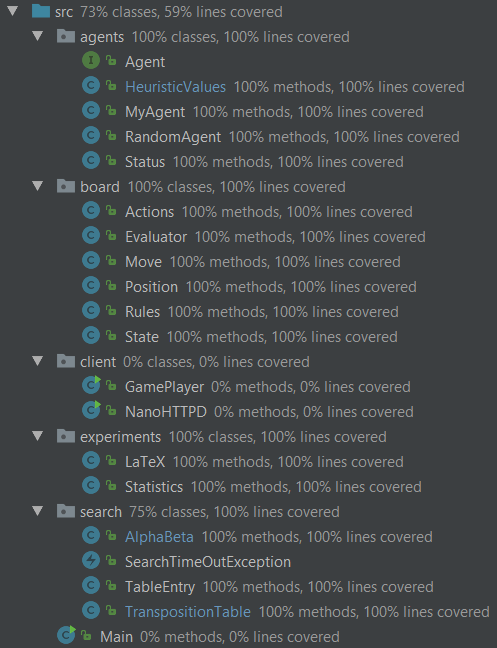
\includegraphics[scale=1]{coverage.png}
\end{center}
\caption{Code coverage}
\label{fig:ccov}
\end{figure}

The following lists the highlights of the tests.
\begin{itemize}
\item Play as white against a random agent 10 times on a $3 \times 5$ board and checking if score is at least 8 (getting 1 for a win, 0 for draw, -1 for a loss). Another test does the same for black.
\item Play as white against a random agent 3 times on a $9 \times 9$ board and checking if we win all. Another test does the same for black.
\item Playing until a game is over as a random agent and check if we return valid commands.
\item Symmetry test for playing as white (white starts) and black (black starts) for two states that are a reflection of each other (about $y=h/2$ or the diagonal), testing heuristics, best move, etc.
\item Testing special case for 'win next' as mentioned in subsection \ref{ss:pe}.
\item Testing if search passes time limit for multiple boards.
\item If various obvious best moves are chosen.
\item All collision cases for transposition tables.
\end{itemize}


\end{document}









